\documentclass[11pt,a4paper]{report}
\usepackage[utf8]{inputenc}
\usepackage[french]{babel}
\usepackage[T1]{fontenc}
\usepackage{amsmath}
\usepackage{amsfonts}
\usepackage{amssymb}
\usepackage{xcolor}
\usepackage{gensymb}

\usepackage{geometry}
\geometry{hmargin=2.5cm,vmargin=1.5cm}
\usepackage{wasysym}
\usepackage{graphicx}

\author{Mathieu Sarrat}
\title{LC10 - Acides et Bases}

\makeatletter
\renewcommand{\thesection}{\@arabic\c@section}
\makeatother


\begin{document}
\maketitle

\section*{Niveau, Pré-requis et objectifs}
\begin{itemize}
	\item \textbf{Niveau :} Terminale S\\
	
	\item \textbf{Pré-requis :}
		\begin{itemize}
			\item Généralités sur le pH
			\item Tableau d'avancement
			\item Fonction logarithme décimal\\
		\end{itemize}
	
	\item \textbf{Objectifs :}
		\begin{itemize}
			\item Définir la notion de pH dans une solution diluée;
			\item Définir les notions d'acide, de base, de couple acido-basique, d'espèce amphotère;
			\item Force des acides et des bases, diagramme de prédominance;
			\item Notion d'équilibre acido-basique.\\
		\end{itemize}
		
	\item \textbf{Recommandations :}
		\begin{itemize}
			\item Faire la gamme de solutions pendant la préparation, refaire un point en direct 						(préparation de la solution, mesure du pH et analyse des résultats)
		\end{itemize}
\end{itemize}

\newpage
\section*{Introduction}

Les espèces chimiques présentant des propriétés acides ou basiques (acido-basiques) sont très présentes dans la vie quotidienne et dans le monde qui nous entoure. Nous allons dans cette leçon reprendre et formaliser un certain nombre de concepts vus dans les années précédentes, notamment les notions de pH, d'acide et de base, au sens de la théorie de Bronsted-Lowry.\\

De nombreuses réactions chimiques ne peuvent pas être considérées comme totales : durant cette leçon, on introduira la notion d'équilibre chimique, atteint lorsque la composition d'un milieu réactionnel n'évolue \textbf{plus}, à travers le contexte des réactions acido-basiques.

\section{Théorie acido-basique de Bronsted-Lowry}

\subsection{Le pH}

Le pH est une grandeur \textbf{sans dimension ni unité} permettant d'\textbf{évaluer quantitativement l'acidité d'une solution aqueuse}. Cette grandeur dépend de la concentration en ions \textbf{oxonium} $\text{H}_3\text{O}^+$, selon la formule
\begin{equation}
	\boxed{\text{pH} = -\text{log}_{10} [\text{H}_3\text{O}^+]} \quad\text{ou encore}\quad 
	\boxed{[\text{H}_3\text{O}^+] = 10^{-\text{pH}}},
\end{equation}
relations qui ne sont valables que si $[\text{H}_3\text{O}^+]\leq 0.1\;\text{mol}.\text{L}^{-1}$.\\

\textbf{Remarque :} la concentration dans le logarithme doit être exprimée en $\text{mol}/\text{L}$.\\

On dit qu'une solution est \textbf{acide} si son pH est inférieur à 7 (donc si la concentration en ions oxonium est telle que $[\text{H}_3\text{O}^+] > 10^{-7} \;\text{mol}.\text{L}^{-1}$), \textbf{basique} s'il est supérieur à 7 ($[\text{H}_3\text{O}^+] < 10^{-7} \;\text{mol}.\text{L}^{-1}$).\\

\textcolor{red}{Manip : mesurer au pH-mètre le pH d'une solution d'acide chlorhydrique à $10^{-2} \;\text{mol}.\text{L}^{-1}$ et calculer la concentration en ions oxonium.}\\

Lorsqu'on dissout un composé dans de l'eau et que son pH diminue, le composé est acide. Si le pH augmente, c'est que le composé est basique.

\subsection{Acide, base, couple acide/base}

\begin{itemize}
	\item Un \textbf{acide} au sens de Bronsted est une espèce susceptible de libérer un proton 
	$\text{H}^+$. Exemple, l'acide méthanoïque (également appelé acide formique car libéré par 				certaines espèces de fourmis lorsqu'elles piquent) :
	\begin{equation}
		\text{HCOOH} = \text{HCOO}^- + \text{H}^+.
		\label{eq:methanoic}
	\end{equation}
	On dit que $\text{HCOO}^-$, l'ion méthanoate, est la \textbf{base conjuguée} de l'acide 				méthanoïque.\\
	Le proton libéré se combine à une molécule d'eau pour donner
	\begin{equation}
		\text{H}^+ + \text{H}_2\text{O} = \text{H}_3\text{O}^+
	\end{equation}
	l'ion oxonium. Ainsi, lorsqu'on ajoute un acide dans l'eau, le pH diminue puisqu'on augmente la 		concentration en ions oxonium.\\
	
	\item Une \textbf{base} au sens de Bronsted est une espèce susceptible de capter un proton. 			Lorsqu'on introduit une base dans l'eau, le pH va donc augmenter puisqu'on va consommer des ions 	oxonium.\\
	Exemple l'ammoniac $\text{NH}_3$, l'un des gaz les plus synthétisés au monde du fait de son 			importance dans la production d'engrais agricole :
	\begin{equation}
		\text{NH}_3 + \text{H}^+ = \text{NH}_4^+.
		\label{eq:ammonium}
	\end{equation}
	L'ion ammonium $\text{NH}_4^+$ est l'acide conjugué de l'ammoniac.\\
\end{itemize}

L'ensemble d'un acide et de sa base conjuguée forme un \textbf{couple acide base}
\begin{equation}
	\text{HCOOH}/\text{HCOO}^-  \quad\text{ou}\quad \text{NH}_4^+/\text{NH}_3.\\
\end{equation}

Si on met en solution l'acide formique et l'ammoniac, ils réagissent pour former leurs espèces conjuguées (on additionne les équations bilan \eqref{eq:ammonium} et \eqref{eq:methanoic} :
\begin{equation}
	\text{HCOOH} + \text{NH}_3 = \text{HCOO}^- + \text{NH}_4^+
\end{equation}

La double flèche signifie que la réaction se fait dans les deux sens : l'acide méthanoïque et l'ammoniac réagissent ensemble, pendant que les produits, l'ion éthanoate et l'ion ammonium, réagissent eux aussi de leur côté.

\subsection{Ampholyte}

Un ampholyte (ou une espèce amphotère) est une espèce qui \textbf{peut se comporter tantôt comme une base, tantôt comme un acide}. C'est notamment le cas de l'eau, qui appartient aux couples
\begin{equation}
	\text{H}_3\text{O}^+ / \text{H}_2\text{O}     \quad\text{et}\quad   
	\text{H}_2\text{O} / \text{HO}^-
\end{equation}
Pour reprendre la terminologie précédente, l'eau est la base conjuguée de l'ion oxonium et l'acide conjugué de l'ion hydroxyde. On a, en effet :
\begin{equation}
	\text{H}_3\text{O}^+ = \text{H}_2\text{O} + \text{H}^+ \quad\text{et}\quad 
	\text{HO}^- + \text{H}^+ = \text{H}_2\text{O}.
\end{equation}

L'eau solvant est en permanence le siège d'une \textbf{réaction d'autoprotolyse}. En effet, l'eau étant à la fois acide et base, une molécule d'eau peut réagir avec une consoeur :
\begin{equation}
	\boxed{2 \text{H}_2\text{O} = \text{H}_3\text{O}^+ + \text{HO}^-}.\\
\end{equation}

Cette réaction montre que dans toute solution aqueuse, il existe des ions oxonium et hydroxyde et leurs concentrations \textbf{exprimées en $\text{mol}.\text{L}^{-1}$} vérifient le \textbf{produit ionique de l'eau} :
\begin{equation}
	\text{K}_\text{e} \equiv [\text{H}_3\text{O}^+] [\text{HO}^-]
\end{equation}
Cette quantité est une constante pour une température donnée. Si $T = 25\degree$C, $K_e = 10^{-14}$. On peut s'en servir pour calculer à tout moment la concentration en ions hydroxyde, connaissant le pH d'une solution. \textcolor{red}{Reprendre la première manip et calculer la concentration en ions hydroxyde correspondante.}\\

\textbf{Remarque :} malgré son expression, $K_e$ n'a pas d'unité. En réalité, on divise chaque concentration par une concentration de 1 $\text{mol}.\text{L}^{-1}$, de sorte que $K_e$ est sans dimension. C'est la même chose pour le pH.\\

L'eau n'est pas la seule espèce chimique amphotère : l'ion hydrogénocarbonate $\text{HCO}_3^-$ est la base conjuguée de l'acide carbonique $\text{H}_2\text{CO}_3$ et l'acide conjugué de l'ion carbonate $\text{CO}_3^{2-}$.

\newpage
\section{Force des acides et des bases}

Comment savoir si un acide est "plus acide" qu'un autre acide ? On veut pouvoir comparer la force des acides et la force des bases.

\subsection{Acide fort et base forte}

Un acide ou une base est qualifié de \textbf{fort} s'il réagit \textbf{totalement avec l'eau}. On fait apparaître une simple flèche, dirigée des réactifs vers les produits, pour souligner le caractère total de la réaction.\\

\textbf{Exemples :}
\begin{itemize}
	\item le \textbf{chlorure d'hydrogène} est un acide fort
	\begin{equation}
		\text{HCl} + \text{H}_2\text{O} \rightarrow \text{Cl}^- + \text{H}_3\text{O}^+.
	\end{equation}
	La solution résultant de cette dissociation est appelée \textbf{acide chlorhydrique}. Il existe 		d'autres acides forts, comme l'iodure d'hydrogène, le bromure d'hydrogène, les acides sulfurique 		et nitrique ...\\
	
	\item \textbf{l'hydroxyde de sodium} (la soude) est une base forte
	\begin{equation}
		\text{NaOH} \rightarrow \text{Na}^+ + \text{HO}^-
	\end{equation}
	Il existe d'autres bases fortes, comme par exemple la potasse (hydroxyde de potassium KOH).\\
\end{itemize}

Dans les deux cas, l'avancement final de la réaction avec l'eau solvant est égal à l'avancement maximal, la \textbf{réaction étant totale}.

\subsection{Réaction entre un acide fort et une base forte}

La réaction entre un acide fort et une base forte est une réaction quasi-totale d'équation
\begin{equation}
	 \text{H}_3\text{O}^+ + \text{HO}^- = \text{H}_2\text{O}.
\end{equation}
Cette réaction est \textbf{exothermique} : elle libère de l'énergie sous forme de chaleur. Pour une mole d'avancement, l'énergie libérée est de l'ordre de 56 kJ à $25\degree$C, soit plus que ce qu'il faut pour augmenter la température d'un kilogramme d'eau de 1 degré. Tout mélange d'un acide fort avec une base forte doit être réalisé avec prudence.\\

\textbf{Remarque :} c'est pour cela qu'on recommande toujours de verser l'acide chlorhydrique concentré dans l'eau, et de ne surtout pas faire le contraire. Des projections auront lieu, compte tenu du caractère très exothermique de la réaction. Si l'eau reçoit l'acide, les projections seront essentiellement constituées d'eau. Si l'eau est versée dans l'acide, ce seront des projections d'acide.\\

\subsection{Acide faible et base faible}

Certains acides et certaines bases ne réagissent que \textbf{partiellement} dans l'eau : la réaction n'est pas totale et on parle d'\textbf{acide faible et de base faible}. Cela signifie qu'\textbf{à la fin de la réaction, toutes les espèces apparaissant dans l'équation bilan sont présentes}.\\

C'est le cas de l'acide éthanoïque $\text{CH}_3\text{COOH}$ (présent dans le vinaigre), qui se dissocie dans l'eau selon la réaction
\begin{equation}
	\text{CH}_3\text{COOH} + \text{H}_2\text{O} \rightleftarrows
	\text{CH}_3\text{COO}^- + \text{H}_3\text{O}^+.
\end{equation} 
La base conjuguée de l'acide éthanoïque est l'ion éthanoate. La double flèche (à simples pointes) traduit l'existence de cet équilibre. La base conjuguée d'un acide faible est une base faible.\\

Parmi les acides faibles, on peut citer l'acide formique rencontré plus haut, l'acide acétylsalicique, principe actif de l'aspirine. De manière générale les acides carboxyliques sont des acides faibles. La molécule d'ammoniac $\text{NH}_3$ est une base faible, de même que les amines.\\

Au bout d'un certain temps, la réaction atteint un \textbf{état d'équilibre} : 
\begin{itemize}
	\item la quantité de matière de toute espèce figurant dans l'équation bilan n'évolue plus;
	\item l'avancement a atteint sa valeur finale, différente de l'avancement maximal qu'on aurait pu 	calculer en supposant la réaction totale.\\
\end{itemize}

On associe à la réaction d'un acide faible dans l'eau une \textbf{grandeur sans unité} appelée \textbf{constante d'acidité}. Dans l'exemple de l'acide éthanoïque, elle s'écrit :
\begin{equation}
	\boxed{\text{K}_\text{a} \equiv \frac{[\text{CH}_3\text{COO}^-][\text{H}_3\text{O}^+]}
	{[\text{CH}_3\text{COOH}]}},
\end{equation}
où les concentrations figurant dans l'expression de $\text{K}_\text{a}$ sont les \textbf{concentrations à l'équilibre, exprimées en $\text{mol}/\text{L}$}. La valeur de $\text{K}_\text{a}$ ne dépend que de la température à laquelle s'effectue la réaction. Comme pour le pH, il est d'usage de définir le $\text{pK}_\text{a}$ d'un couple acido-basique :
\begin{equation}
	\boxed{\text{pK}_\text{a} \equiv -\text{log}_{10}\;\text{K}_\text{a}}.
\end{equation}

Plus le $\text{pK}_\text{a}$ est petit, plus la constante d'acidité est grande, plus l'acide est dissocié (avancement plus grand) et plus il acidifie la solution. Les $\text{pK}_\text{a}$ permettent donc de comparer l'avancement final de la réaction de différents acides faibles dans l'eau, et donc de comparer leur force. La comparaison se fait pour une concentration totale $[\text{AH}] + [\text{A}^-]$ donnée.

\begin{figure}[h!]
	\begin{center}
  		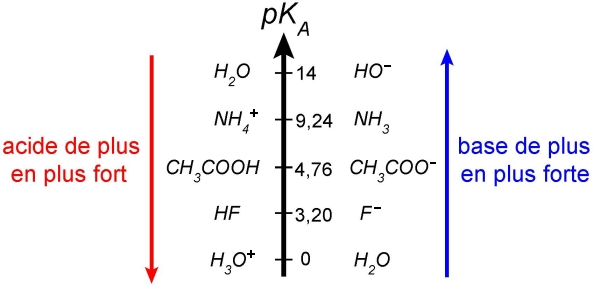
\includegraphics[scale = 0.7]{pkascaling.png}
	\caption{Échelle de pKa pour quelques couples acide base.}
	\end{center}
\end{figure}

\subsection{Diagrammes de prédominance}

En utilisant le logarithme décimal sur l'équation définissant la constante d'acidité, on obtient
\begin{equation}
	\text{log}_{10}\;\text{K}_\text{a} = \text{log}_{10}[\text{H}_3\text{O}^+] 
	+ \text{log}_{10}\frac{[\text{CH}_3\text{COO}^-]}{[\text{CH}_3\text{COOH}]}
\end{equation}
que l'on réécrit
\begin{equation}
	\text{pH} = \text{pK}_\text{a} 
	+ \text{log}_{10}\frac{[\text{CH}_3\text{COO}^-]}{[\text{CH}_3\text{COOH}]}.
\end{equation}

Si les concentrations en acide et en base conjuguée sont les mêmes, on remarque que 
\begin{equation}
	\text{pH} = \text{pK}_\text{a}. 
\end{equation}
Dans le cas où $\text{pH} < \text{pK}_\text{a}$, on dit que la forme acide prédomine puisque dans ce cas $[\text{CH}_3\text{COO}^-] < [\text{CH}_3\text{COOH}]$. Dans le cas où $\text{pH} > \text{pK}_\text{a}$, c'est la forme basique qui prédomine.\\

\newpage
\textbf{Détermination expérimentale du $\text{pK}_\text{a}$ de l'acide éthanoïque}
\begin{itemize}
	\item Le Maréchal, Chimie Générale p9.
	\item Dresser un tableau d'avancement (on introduit dès le début acide et base conjuguée), faire l'hypothèse que les concentrations vont peu varier, on peut donc tracer la courbe pH en fonction du logarithme du rapport des concentrations en gardant les concentrations initiales.\\ 
\end{itemize}

\textbf{Discuter la prédominance de l'acide et de la base dans le cas de l'acide éthanoïque pour clore cette partie.}

\section{Acides et bases}

\subsection{Les acides alpha-aminés}

Les acides $\alpha-$aminés sont des composés dont l'un des atomes de carbone porte une fonction carboxyle et une fonction amine. Ce sont les briques fondamentales constituant les protéines: certains sont qualifiés d'\textbf{essentiels}, c'est-à-dire que le corps ne peut les synthétiser et qu'il doit se les procurer par l'alimentation.\\

Ces molécules possèdent des propriétés acido-basiques. Ils sont en effet capables de perdre deux protons et sont donc caractérisés par deux valeurs de $\text{pK}_\text{a}$ :
\begin{itemize}
	\item le plus petit correspond au couple $\text{RCOOH}/\text{RCOO}^-$,
	\item le plus grand correspond au couple $\text{RNH}_3^+/\text{RNH}_2$.\\
\end{itemize}

\begin{figure}[h!]
	\begin{center}
		\begin{tabular}{cc}
  		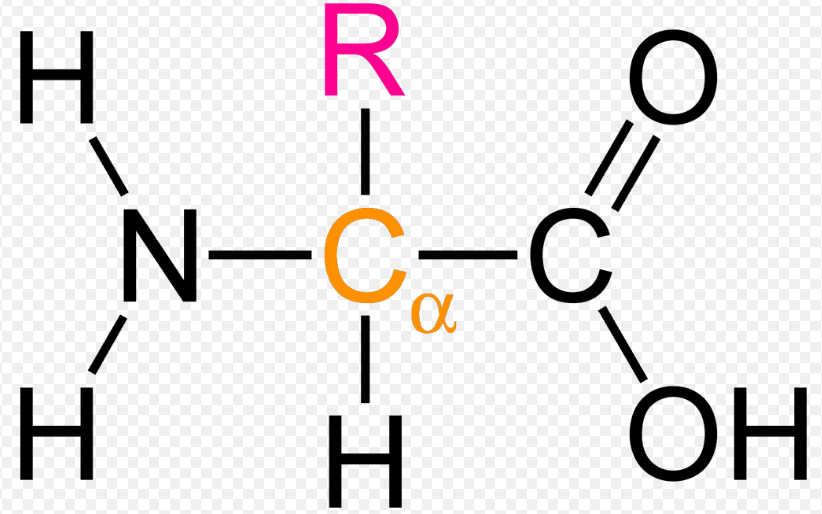
\includegraphics[scale = 0.20]{alpha_amine.png} &
   		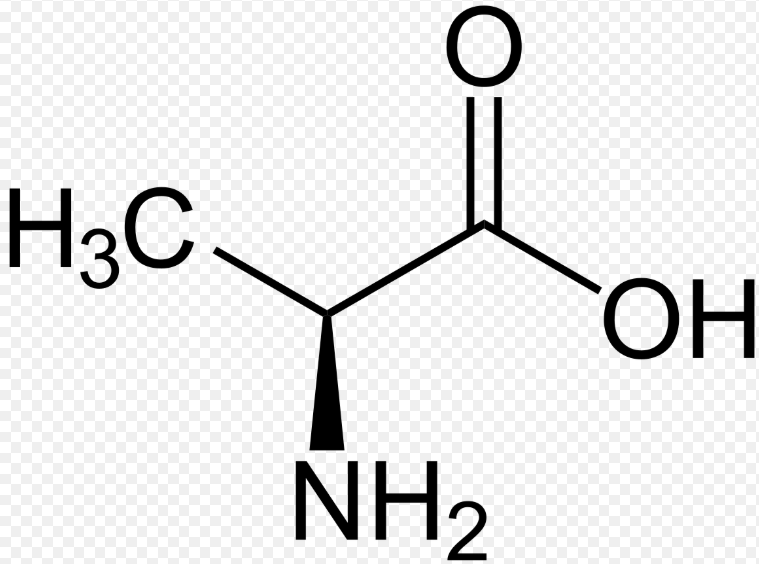
\includegraphics[scale = 0.20]{alanine.png}\\
	\end{tabular}
	\caption{Gauche : forme générale d'un acide $\alpha-$aminé. Droite : l'alanine.}
	\end{center}
\end{figure}

Intéressons-nous au cas de l'alanine, dont nous allons tracer le diagramme de prédominance ($\text{pK}_\text{a} = 2.35 \text{et} 9.87$) :
\begin{equation}
	\text{CH}_3-\text{CH(NH}_3^+) -\text{COOH} 
	= \text{H}^+ + \text{CH}_3-\text{CH(NH}_3^+)-\text{COO}^-
\end{equation}
\begin{equation}
	\text{CH}_3-\text{CH(NH}_3^+)-\text{COO}^-
	= \text{H}^+ + \text{CH}_3-\text{CH(NH}_2)-\text{COO}^-
\end{equation}

La forme intermédiaire, présentant une charge positive et une charge négative simultanément, est amphotère et on l'appelle \textbf{zwitterion}. 

\subsection{Pouvoir tampon}

La présence simultanée, \textbf{en quantités comparables} des formes acide et basique d'un couple acido-basique empêche le pH de varier sensiblement lors :
\begin{itemize}
	\item d'un ajout modéré d'acide fort ou de base forte,
	\item d'une dilution.
\end{itemize}

Une telle solution est qualifiée de \textbf{solution tampon}, efficace dans un intervalle de pH $+1/-1$ situé autour du pKa du couple.\\

La régulation du pH sanguin (\textbf{équilibre acido-basique} en physiologie) est essentielle à la survie de l'organisme. Il varie normalement entre 7,38 et 7,42 (légèrement basique). S'il descend trop bas, on parle d'\textbf{acidose}, s'il grimpe trop haut, on parle d'\textbf{alcalose}.\\

Le couple $\text{HCO}_3^-/\text{CO}_3^{2-}, \text{pKa} = 10.3$ (ion hydrogénocarbonate/ion carbonate) est le principal couple responsable du maintien du pH sanguin par son action tampon. L'ion hydrogénocarbonate est une espèce amphotère, base conjuguée du dioxyde de carbone ($\text{CO}_2/\text{HCO}_3^-$, $\text{pKa} = 6.4$).\\

En cas d'effort intense, ce pouvoir tampon ne suffit plus et l'organisme puise dans ses réserves d'énergie en oxydant le glucose
\begin{equation}
	\text{C}_6\text{H}_{12}\text{O}_6 + 6\;\text{O}_{2} 
	\rightarrow 6\;\text{CO}_{2} + 6\;\text{H}_2\text{O}.
\end{equation}	
Cette oxydation produit du dioxyde de carbone, espèce acide faible, transportée par le sang jusqu'aux poumons où elle est évacuée de l'organisme. Le dioxyde de carbone réagit avec l'eau selon la réaction
\begin{equation}
	\text{CO}_{2} + 2\;\text{H}_2\text{O} \rightleftarrows
	\text{HCO}_3^- + \text{H}_3\text{O}^+
\end{equation}
Si trop de dioxyde de carbone est produit, la régulation par le tampon hydrogénocarbonate/carbonate ne suffit plus, et l'organisme déclenche un autre mécanisme : il augmente le rythme de la respiration pour évacuer ce gaz plus efficacement.\\

\begin{figure}[h!]
	\begin{center}
		\begin{tabular}{cc}
  		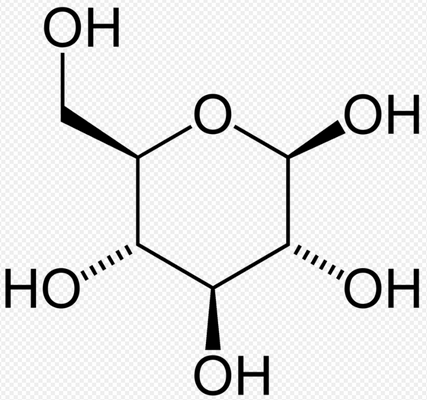
\includegraphics[scale = 0.20]{glucose.png} &
   		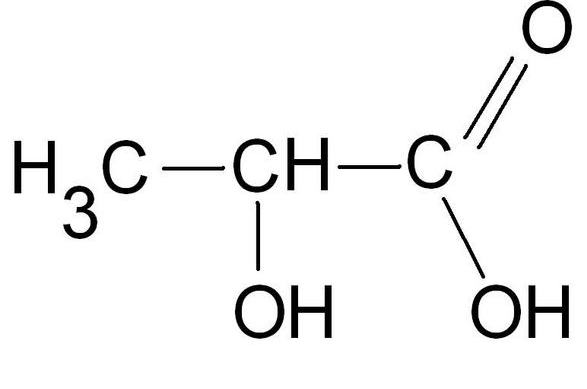
\includegraphics[scale = 0.20]{acide_lactique.png}\\
	\end{tabular}
	\caption{Gauche : glucose. Droite : acide lactique.}
	\end{center}
\end{figure}

Si la ventilation pulmonaire est insuffisante, l'oxydation du glucose n'est que partielle et conduit à la formation d'acide lactique (pKa $= 3.90$, l'ion lactate étant la base conjuguée), responsable de crampes musculaires.

\subsection{Effervescence de l'aspirine}

L'Aspirine, dont le principe actif est l'acide acétylsalicylique (un acide faible, $\text{pKa} = 3.86$ est l'un des principaux médicaments consommés à notre époque. On peut la trouver sous \textbf{forme effervescente} : les excipients sont essentiellement l'acide citrique et l'hydrogénocarbonate de sodium.\\ 

L'acide citrique est ce que l'on appelle un polyacide, comme les acides-aminés. Il est capable de libérer trois protons et est donc caractérisé par trois valeurs de $\text{pKa} = 3.13, 4.76$ et $6.40$. Dans l'eau ($pH = 7$), les trois protons de l'acide citrique sont libérés. L'acide acétylsalicylique est caractérisé par un $\text{pKa} = 2.9$.\\ 

Lorsqu'on introduit un cachet dans l'eau, on déclenche \textbf{une réaction acido-basique entre l'acide citrique et les ions hydrogénocarbonate} (couples $\text{H}_3\text{Citr}/\text{Citr}^{3-}$ (simplifié, il y en a 3) et $\text{CO}_2/\text{HCO}_3^-$).
\begin{equation}
\text{H}_3\text{Citr}+3\;\text{HCO}_3^-=\text{Citr}^{3-}+3\;\text{H}_2\text{O}+3\;\text{CO}_{2(g)}
\end{equation}
(bilan global) produisant du dioxyde de carbone gazeux, d'où l'effervescence.\\

\begin{figure}[h!]
	\begin{center}
		\begin{tabular}{cc}
  		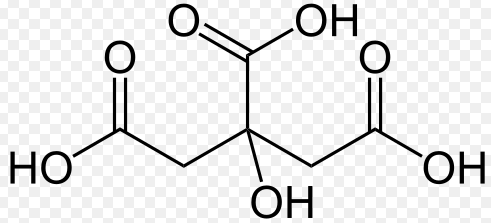
\includegraphics[scale = 0.50]{acide_citrique.png} &
   		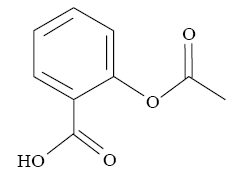
\includegraphics[scale = 0.50]{acide_acetylsalicylique.png}\\
	\end{tabular}
	\caption{Gauche : acide citrique. Droite : acide acétylsalicylique.}
	\end{center}
\end{figure}

\begin{figure}[h!]
	\begin{center}
  		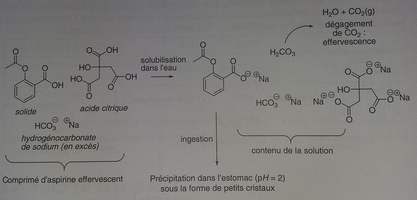
\includegraphics[scale = 0.8]{effervescence.png}
	\caption{Effervescence de l'aspirine.}
	\end{center}
\end{figure}

\textbf{Diagramme de prédominance de l'acide acétylsalicylique} : dans le verra d'eau l'aspirine est présente sous forme ionique : l'ion acétylsalicylate (l'aspirine tamponnée est à $\text{pH} \simeq 6,4$, bien plus soluble dans l'eau que l'acide acétylsalicylique. Dans l'estomac, le pH est de l'ordre de 2 au beau milieu de la digestion. L'ion acétylsalicylate va capter des protons et revenir sous forme acide, où il va reformer de petits cristaux, plus facilement assimilables par l'organisme que si on avait ingéré l'acide sous forme non tamponée.


\newpage
\section*{Conclusion}

\newpage
\section*{Annexes}

\subsubsection*{Protéines}

Les protéines sont des macromolécules biologiques présentes dans toutes les cellules vivantes. Elles sont formées d'une ou de plusieurs chaînes polypeptidiques. Chacune de ces chaînes est constituée de l'enchaînement de résidus d'acides aminés liés entre eux par des liaisons peptidiques :

\begin{itemize}
	\item \textbf{Liaison peptidique :}
	La liaison est le résultat de la réaction entre la fonction acide carboxylique $\text{COOH}$ du 		premier acide aminé et la fonction amine $\text{NH}_2$ du deuxième, avec comme produit secondaire 	une molécule d'eau.
	\begin{figure}[h!]
		\begin{center}
		\begin{tabular}{cc}
  			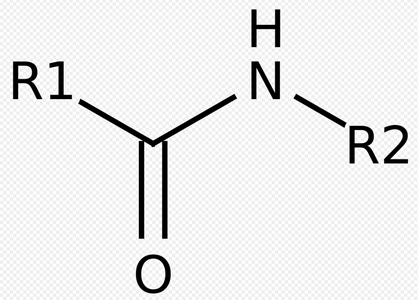
\includegraphics[scale = 0.5]{liaison_peptidique.png} &
   			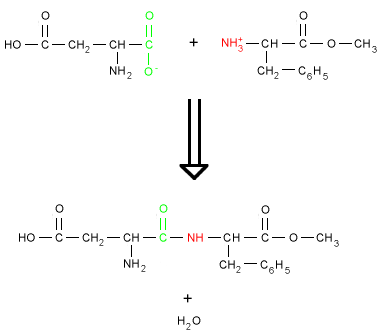
\includegraphics[scale = 0.9]{formation_peptidique.png}\\
		\end{tabular}
		\caption{Gauche : forme générale d'un acide $\alpha-$aminé. Droite : la glycine est le plus 			simple d'entre eux, représentée ici sous forme de zwitterion.}
		\end{center}
	\end{figure}
	
	\item \textbf{Structure des protéines :} quatre niveaux d'organisation
	\begin{itemize}
		\item \textbf{Structure primaire} : séquence en acides aminés;
		\item \textbf{Structure secondaire} : arrangement locaux des acides aminés, 								\textbf{stabilisées par des liaisons hydrogène}, hélices $\alpha$ et feuillets $\beta$;
		\item \textbf{Structure tertiaire} : forme générale de la protéine observable à l'échelle de 				la molécule tout entière (repliement d'une protéine);
		\item \textbf{Structure quaternaire} : complexe résultant de l'assemblage de plusieurs 						molécules de protéines (plusieurs chaînes polypeptidiques), appelées dans ce cas sous-					unités protéiques, pour former un complexe protéique unique. Toutes les protéines ne sont 			pas nécessairement constituées de plusieurs sous-unités et ne possèdent par conséquent 					pas toujours de structure quaternaire.
	\end{itemize}
\end{itemize}

\end{document}